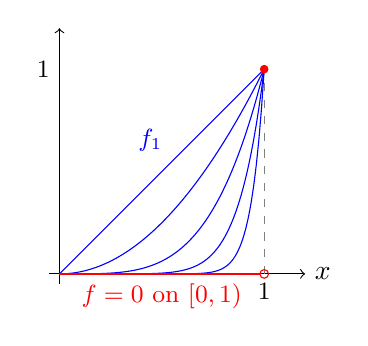
\begin{tikzpicture}[scale=2.6]
  \draw[->] (-0.05,0) -- (1.2,0) node[right] {$x$};
  \draw[->] (0,-0.05) -- (0,1.2);
  \foreach \n in {1,2,4,8,16} {
    \draw[blue, domain=0:1, samples=80] plot (\x, {\x^\n});
  }
  \node[blue, above left] at (0.55,0.55) {\small $f_1$};
  \fill (1,1) circle (0.5pt);
  \draw[dashed, gray] (1,0) -- (1,1);
  \node[below] at (1,0) {\small $1$};
  \node[left] at (0,1) {\small $1$};
  \draw[red, thick] (0,0) -- (0.98,0);
  \fill[red] (1,1) circle (0.6pt);
  \draw[red] (1,0) circle (0.6pt);
  \node[red, below] at (0.5,0) {\small $f=0$ on $[0,1)$};
\end{tikzpicture}
